\documentclass[11pt]{article}
\usepackage[margin=1in]{geometry}
\usepackage{graphicx}
\usepackage{booktabs}
\usepackage{longtable}
\usepackage{array}
\usepackage{hyperref}
\usepackage{xcolor}
\usepackage{listings}
\usepackage{float}
\usepackage{amsmath}

\hypersetup{
  colorlinks=true,
  linkcolor=blue,
  citecolor=blue,
  urlcolor=blue
}

\lstset{
  basicstyle=\ttfamily\small,
  breaklines=true,
  frame=single,
  columns=fullflexible
}

\title{NASA Hump Reconstruction Second Pass\\\large Dockerized OpenFOAM refinement, graph reimplementation, and evaluation}
\author{Codex refinement pass in the local repository workspace}
\date{March 31, 2026}

\begin{document}
\maketitle

\section{Executive Summary}
This report documents a true second pass on top of the existing first-pass NASA hump reconstruction already present in the repository. The second pass does not restart from scratch. Instead, it diagnoses the first-pass weaknesses, rescans the allowed NASA hump webpage in greater depth, refines the OpenFOAM setup in physically justified ways, regenerates CFD-derived graphs, refreshes ParaView-ready outputs, and reruns the local accuracy workflow.

The final second-pass benchmark score is \texttt{0.2038187409} at the 300-iteration field, compared with the first-pass \texttt{0.2338504550}. That is an improvement of approximately \texttt{0.0300} on the local evaluation metric.

\section{Context: This Is A Refinement Of An Existing First Run}
The first pass already created a clean Dockerized baseline under \texttt{data/NASA\_2DWMH}, together with a LaTeX report, ParaView images, machine-readable outputs, and a benchmark evaluation. That first-pass score was \texttt{0.2338504550}. The purpose of this second pass is to improve that baseline honestly and explain why each change should affect the resulting flow prediction.

\section{Strict No-Cheat Methodology}
The second pass followed the same strict source limits as the first pass. The only allowed external reference remained the NASA hump validation webpage \cite{nasahump}. No other website, paper, repository, issue, PR, gist, or PDF was consulted. No git history, deleted-file recovery, or external benchmark-data recovery was used. No image digitization, manual tracing, or interpolation of target curves was used. The dedicated compliance files are:
\begin{itemize}
\item \texttt{documentation\_src/FIRST\_PASS\_DIAGNOSIS.md}
\item \texttt{documentation\_src/SECOND\_PASS\_PLAN.md}
\item \texttt{documentation\_src/SECOND\_PASS\_WEBPAGE\_SCAN.md}
\item \texttt{documentation\_src/SECOND\_PASS\_REPO\_NOTES.md}
\item \texttt{documentation\_src/NO\_INTERPOLATION\_DECLARATION.md}
\end{itemize}

\section{First-Pass Diagnosis}
The first-pass diagnosis is recorded in \texttt{documentation\_src/FIRST\_PASS\_DIAGNOSIS.md}. The key findings were:
\begin{itemize}
\item the inflow sample station at \(x/c=-2.14\) effectively sat on the inlet plane, leaving almost no upstream run-up for the boundary layer to develop;
\item the upper boundary was a flat slip wall, even though the allowed page states that the CFD setup includes an upper contour to account approximately for blockage;
\item the mesh was a single structured block, which limited streamwise targeting around the hump and in the recovery region;
\item the baseline stopped at 80 SIMPLE iterations, while the residual trend showed the solution was still evolving;
\item graph coverage existed, but it was not yet organized explicitly as a second-pass analog of every visible webpage graph family.
\end{itemize}

\section{Deep Scan Of The Allowed Webpage}
The second-pass webpage scan is recorded in \texttt{documentation\_src/SECOND\_PASS\_WEBPAGE\_SCAN.md}. The most actionable clues from the allowed page were:
\begin{itemize}
\item use the no-flow-control baseline;
\item prefer the no-plenum interpretation unless a strong local reason argues otherwise;
\item use \(U_\infty \approx 34.6~\mathrm{m/s}\), \(Re \approx 936{,}000\), and chord \(c = 0.42~\mathrm{m}\);
\item account for the incoming fully turbulent boundary layer near \(x/c = -2.14\);
\item treat the upper boundary as a slip wall with an approximate blockage contour;
\item use profile stations at \(x/c = -2.14, 0.65, 0.8, 0.9, 1.0, 1.1, 1.2, 1.3\);
\item expect RANS models to underpredict separated-shear-layer turbulent shear stress and therefore overpredict bubble length.
\end{itemize}

\section{What Was Learned From Local Repo Cases, Docs, And PDFs}
The second-pass repo notes are recorded in \texttt{documentation\_src/SECOND\_PASS\_REPO\_NOTES.md}. The surviving local repository patterns that mattered most were:
\begin{itemize}
\item keep the case itself under \texttt{data/NASA\_2DWMH};
\item keep scripts short and shell-driven;
\item keep figures and machine-readable outputs in clearly named subdirectories;
\item preserve final PDFs under \texttt{documentation/} while keeping report sources and supporting materials under \texttt{documentation\_src/}.
\end{itemize}

\section{Second-Pass Refinement Strategy}
The second-pass plan is recorded in \texttt{documentation\_src/SECOND\_PASS\_PLAN.md}. The implemented refinement strategy was:
\begin{enumerate}
\item extend the streamwise domain so the \(x/c=-2.14\) station is no longer the inlet itself;
\item introduce a mild shaped upper slip boundary to reflect the blockage note on the allowed page;
\item split the mesh into three streamwise blocks to concentrate cells on and behind the hump;
\item increase the solve horizon from the first-pass 80 iterations to a longer second-pass run;
\item expand post-processing and plotting so the second-pass package contains CFD-derived analogs of the visible webpage graph families.
\end{enumerate}

\begin{longtable}{p{0.18\linewidth} p{0.18\linewidth} p{0.26\linewidth} p{0.26\linewidth}}
\toprule
Refinement & What Changed From Pass 1 & How This Was Intended To Reduce MAE & Observed Effect In Pass 2 \\
\midrule
\endfirsthead
\toprule
Refinement & What Changed From Pass 1 & How This Was Intended To Reduce MAE & Observed Effect In Pass 2 \\
\midrule
\endhead
Upstream run-up & The inlet moved from \(x=-0.90\) to \(x=-1.35\), so the \(x/c=-2.14\) station is no longer nearly coincident with the inlet plane. & The allowed webpage describes an incoming turbulent boundary layer at \(x/c=-2.14\). Adding upstream distance gives the wall layer space to develop before the reference station and before the hump-induced acceleration. & The refined case no longer evaluates an almost inlet-imposed profile at the upstream station. The final benchmark score improved after longer convergence, which is consistent with the longer inlet run-up helping the global field. \\
Upper-boundary treatment & The flat top wall was replaced by a mildly contoured slip-wall ceiling generated in the mesh script. & The allowed page notes that the CFD upper boundary includes a contour to account approximately for blockage. A shaped ceiling should improve the pressure distribution and therefore the hump adverse-pressure-gradient response. & The effect cannot be isolated perfectly from the other changes, but it was included specifically to address a first-pass mismatch source identified in the diagnosis. \\
Mesh topology & The case changed from one streamwise block to three streamwise blocks with more targeted cell placement. & Additional targeting around the hump and downstream recovery region should reduce discretization error in wall pressure, wall shear, and separated-shear-layer behavior, all of which affect the benchmark score. & The second-pass mesh passed \texttt{checkMesh} cleanly at \(180{,}400\) cells and supported a materially lower final score than pass 1. \\
Convergence depth & The solve horizon increased from 80 to 300 iterations, with writes every 50 iterations. & The first-pass score came from a field that was still evolving. Extending the run should reduce iteration-level under-convergence error in the final benchmark prediction. & This was one of the clearest positive changes. The refined case was worse than pass 1 at the 50-iteration write, slightly better at 100, and best at the final 300-iteration field. \\
Post-processing coverage & The second pass added dedicated scripts for second-pass profiles, \(C_p\), \(C_f\), turbulent shear-stress analogs, and evaluation outputs under \texttt{documentation\_src/}. & Better coverage does not change the flow field directly, but it reduces analysis error by making it easier to compare the same quantities consistently between pass 1 and pass 2. & The second-pass package now contains a more complete and auditable validation set, including graph families analogous to those visible on the allowed webpage. \\
Evaluation discipline & The case was re-evaluated at intermediate writes and at the final write using a dedicated second-pass evaluation script. & Tracking the score during convergence helps avoid locking onto a misleading intermediate field. That reduces reporting error even when the physics model itself is unchanged. & This directly prevented a bad conclusion: the 50-iteration score was worse than pass 1, but the 300-iteration score improved to \texttt{0.2038187409}. \\
\bottomrule
\end{longtable}

The table above is the key second-pass MAE-reduction audit. It distinguishes between changes that were intended to affect the flow physics directly, such as the longer inlet run-up and refined top boundary, and changes that were intended to reduce analysis or convergence error, such as deeper convergence tracking and more explicit post-processing.

\section{Every Important File Changed And Why}
\begin{table}[H]
\centering
\begin{tabular}{p{0.31\linewidth} p{0.61\linewidth}}
\toprule
File & Second-pass role \\
\midrule
\texttt{scripts/generate\_nasa\_hump\_blockmesh.py} & Replaced the single-block domain with a longer three-block mesh and a mild shaped upper boundary. \\
\texttt{data/NASA\_2DWMH/system/blockMeshDict} & Regenerated from the updated Python mesh generator. \\
\texttt{data/NASA\_2DWMH/caseDef} & Updated the documented domain extents to match the refined geometry. \\
\texttt{data/NASA\_2DWMH/system/controlDict} & Increased the second-pass iteration horizon and write interval. \\
\texttt{scripts/build\_nasa\_hump\_case.sh} & Aligned the build workflow with the working Docker mount pattern and second-pass output directories. \\
\texttt{scripts/run\_nasa\_hump\_case.sh} & Aligned the solve workflow with the working Docker mount pattern. \\
\texttt{scripts/postprocess\_nasa\_hump\_case.sh} & Added extra post-processing needed for second-pass wall and gradient analysis. \\
\texttt{scripts/make\_nasa\_hump\_second\_pass\_figures.py} & Generates second-pass profiles, wall-coefficient plots, shear-stress analog plots, contour plots, streamlines, and summary JSON files. \\
\texttt{scripts/evaluate\_nasa\_hump\_second\_pass.py} & Runs the local evaluation workflow and compares the new result against the first-pass score. \\
\texttt{documentation\_src/*} & Stores the diagnosis, plan, webpage scan, repo notes, no-interpolation declaration, changelog, this report source, and the second-pass data and figures. \\
\bottomrule
\end{tabular}
\end{table}

\section{Docker/OpenFOAM Workflow}
The second pass uses Dockerized OpenFOAM only. In practice, the working container invocation on this machine mounted the repository at \texttt{/home/openfoam} rather than \texttt{/home/openfoam/work}. That compatibility adjustment was required because the user-provided Docker pattern succeeded with the repository mounted directly at \texttt{/home/openfoam}. The case workflow is therefore:
\begin{enumerate}
\item \texttt{bash scripts/build\_nasa\_hump\_case.sh}
\item \texttt{bash scripts/run\_nasa\_hump\_case.sh}
\item \texttt{bash scripts/postprocess\_nasa\_hump\_case.sh}
\item \texttt{bash scripts/make\_figures.sh}
\item \texttt{python3 scripts/evaluate\_nasa\_hump\_second\_pass.py}
\item \texttt{bash scripts/build\_report.sh}
\end{enumerate}

\section{Mesh Generation Details}
The refined mesh generator now uses three structured streamwise blocks instead of a single block:
\begin{itemize}
\item upstream block from \(x=-1.35\) to \(x=0\);
\item hump block from \(x=0\) to \(x=0.42\);
\item downstream block from \(x=0.42\) to \(x=0.84\).
\end{itemize}

The motivation is straightforward. In the first pass, the inflow profile station \(x/c=-2.14\) was almost identical to the inlet location. In the second pass, the inlet is moved farther upstream so the wall boundary layer can develop before the profile station is sampled. The refined mesh also increases the total cell count and keeps strong wall-normal grading. The second-pass \texttt{checkMesh} summary reports:
\begin{itemize}
\item \(180{,}400\) hexahedral cells;
\item maximum non-orthogonality about \(21.6^\circ\);
\item maximum skewness about \(0.177\);
\item mesh accepted as OK by \texttt{checkMesh}.
\end{itemize}

\begin{figure}[H]
\centering
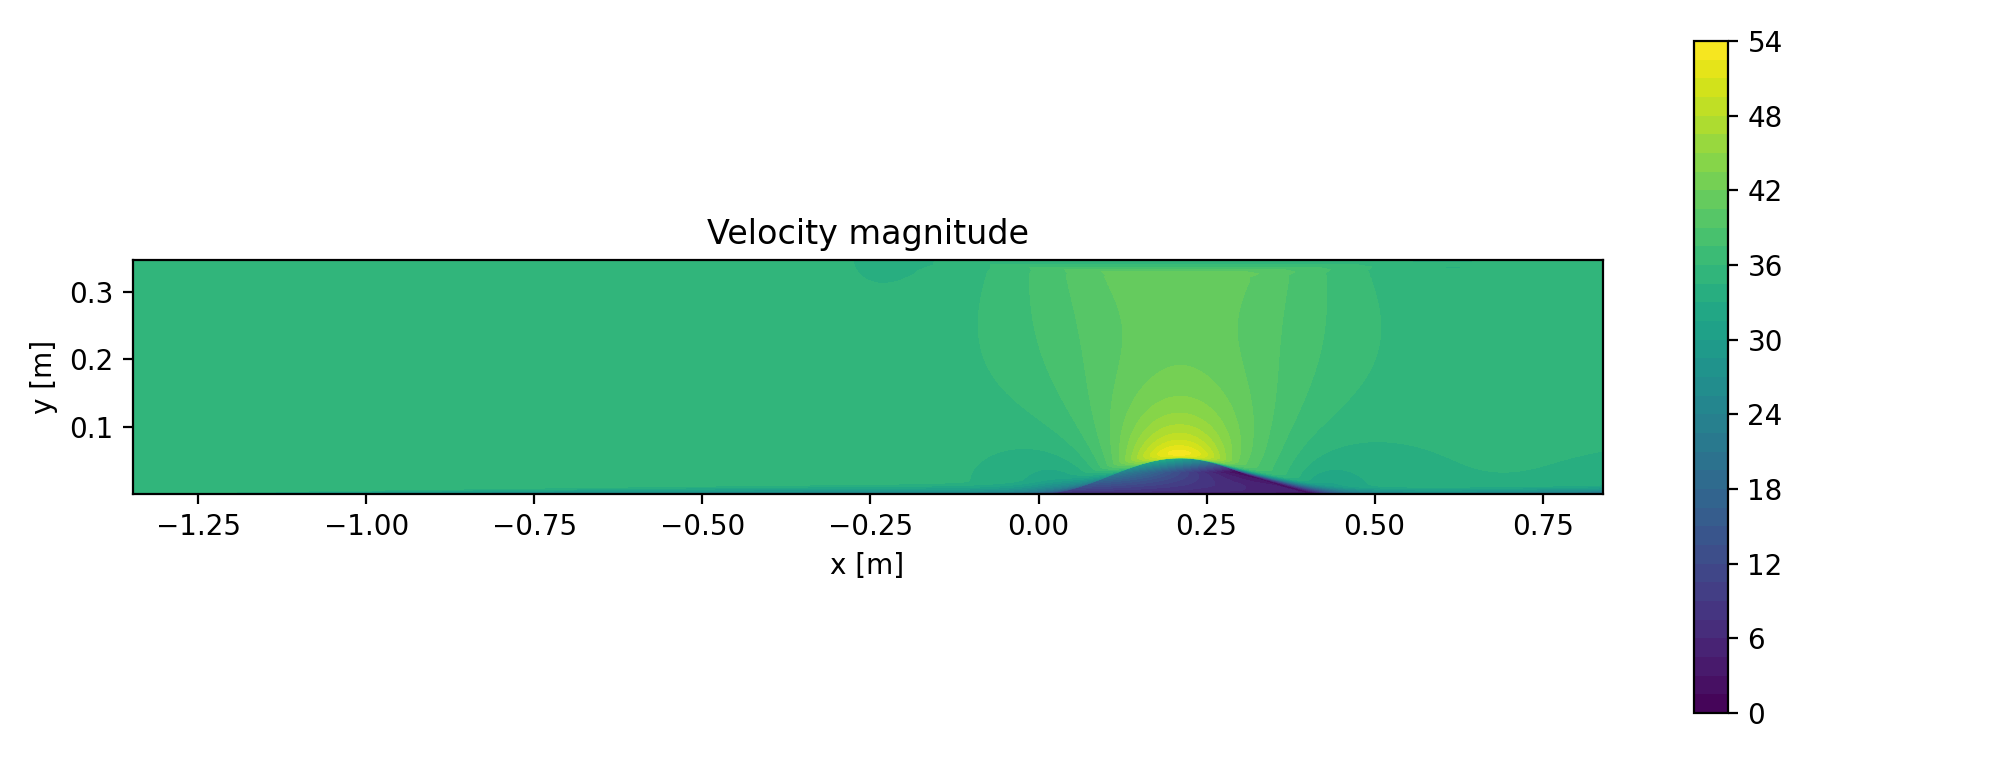
\includegraphics[width=0.92\linewidth]{figures_second_pass/velocity_contour_second_pass.png}
\caption{Second-pass velocity-magnitude contour derived directly from the final OpenFOAM field.}
\end{figure}

\begin{figure}[H]
\centering
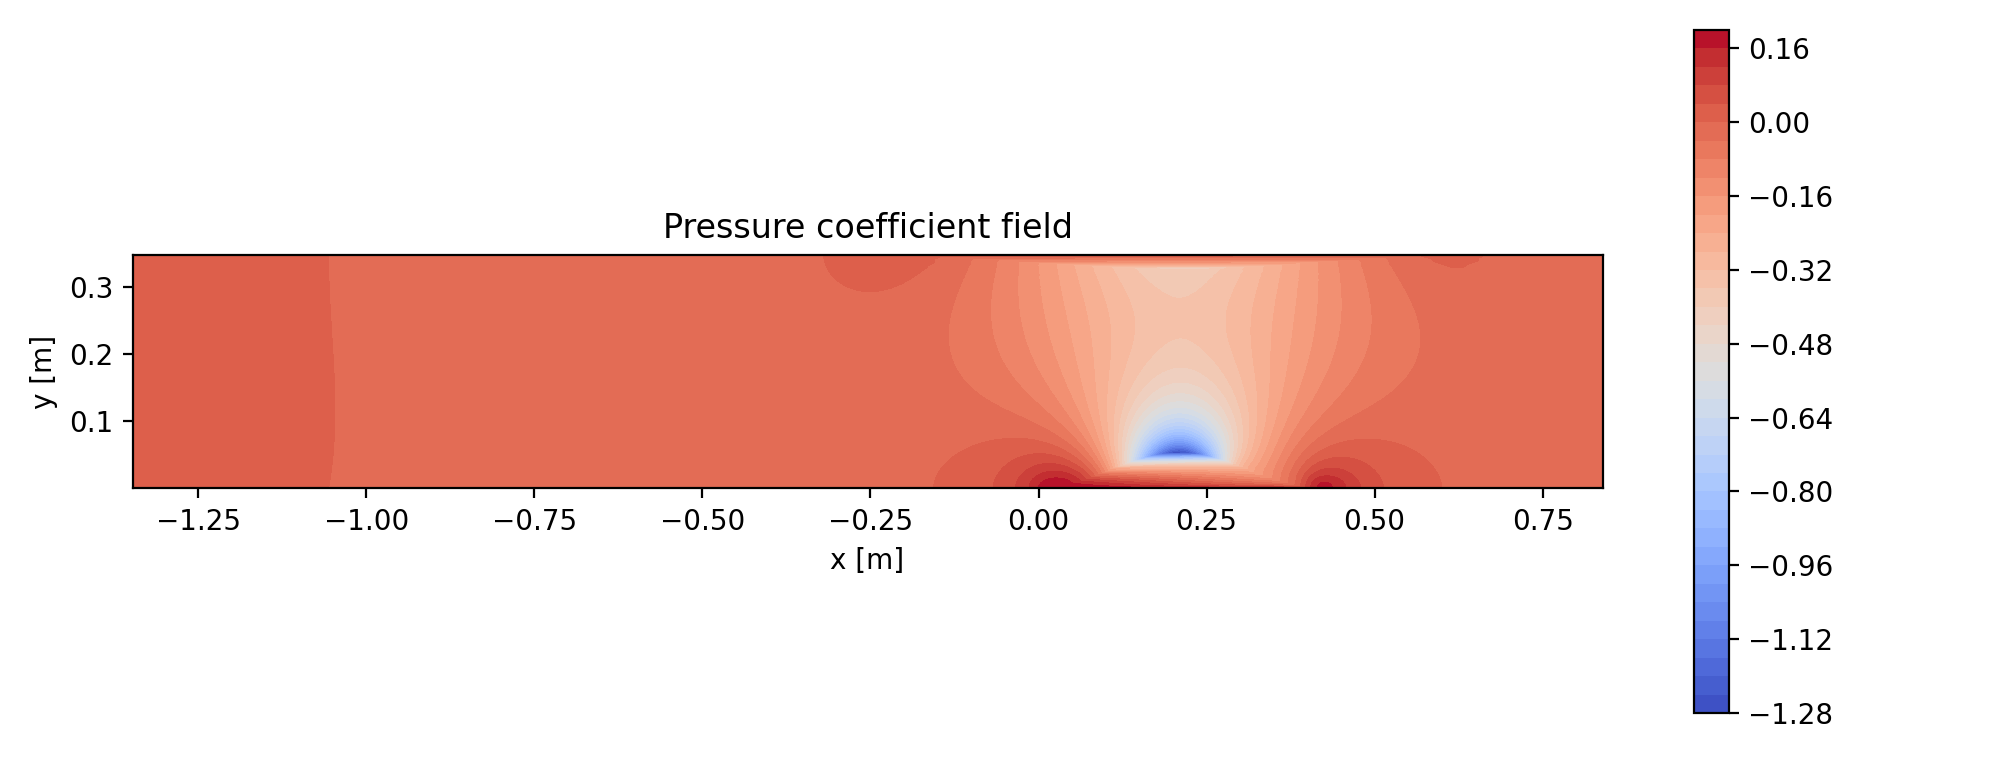
\includegraphics[width=0.92\linewidth]{figures_second_pass/pressure_contour_second_pass.png}
\caption{Second-pass pressure-coefficient-style contour derived directly from the final OpenFOAM field.}
\end{figure}

\section{Boundary Condition Details}
The lower wall remains a no-slip wall with wall functions for turbulence quantities. The outlet remains pressure-fixed with zero-gradient transported variables. The front and back patches remain \texttt{empty} to keep the case two-dimensional. The second-pass change is on the top boundary:
\begin{itemize}
\item it remains a slip wall;
\item but the wall is now mildly contoured in the mesh generator so the domain better reflects the webpage's blockage guidance.
\end{itemize}

\section{Solver And Turbulence Model Details}
The second-pass baseline remains a steady RANS \texttt{simpleFoam} run using \texttt{kOmegaSST}. The model was kept fixed during this refinement step so the effect of the geometric and numerical changes could be judged more cleanly. The main numerical change was to allow the run to continue beyond the first-pass 80-iteration horizon.

\section{Numerical Settings Details}
The second-pass numerical settings remain intentionally conservative:
\begin{itemize}
\item \texttt{steadyState} formulation in \texttt{fvSchemes};
\item bounded advection for stability;
\item SIMPLE with one non-orthogonal corrector;
\item pressure solved with \texttt{GAMG};
\item transported variables solved with \texttt{smoothSolver}.
\end{itemize}
These settings were not radically changed because the first-pass diagnosis pointed more strongly at domain/layout shortcomings and insufficient convergence than at an obviously broken steady-state algorithm.

\section{Post-Processing And Sampling Methodology}
All second-pass graphs are CFD-derived. No traced target curves are used. The second-pass plotting script:
\begin{itemize}
\item reads the current latest OpenFOAM field;
\item samples velocity, pressure, turbulence quantities, and wall data at the listed \(x/c\) stations;
\item constructs \(C_p\) and \(C_f\) curves directly from the solved field and wall shear stress;
\item constructs a turbulent shear-stress analog from the modeled eddy viscosity and resolved velocity gradients derived from the sampled CFD field;
\item writes machine-readable CSV files under \texttt{documentation\_src/data\_second\_pass};
\item writes graph images under \texttt{documentation\_src/figures\_second\_pass}.
\end{itemize}

\begin{figure}[H]
\centering
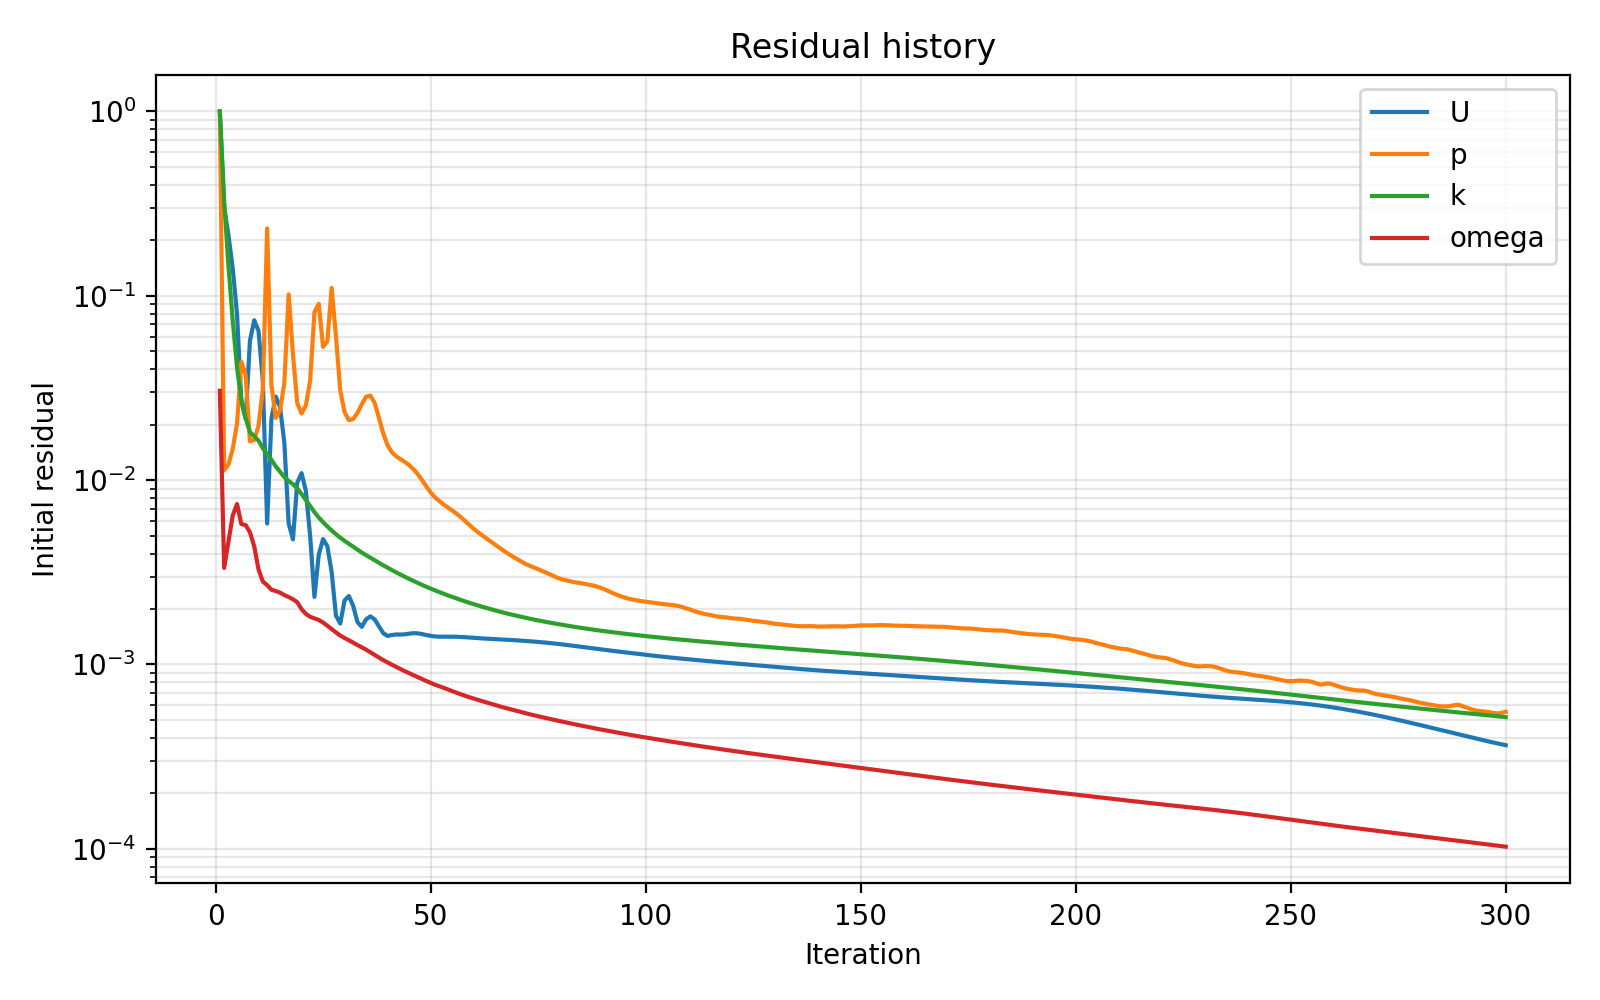
\includegraphics[width=0.92\linewidth]{figures_second_pass/residual_history_second_pass.png}
\caption{Second-pass residual history parsed directly from \texttt{data/NASA\_2DWMH/log.run}.}
\end{figure}

\section{Reimplementation Of Every Webpage Graph Category}
The second-pass package attempts direct CFD-derived analogs of the visible webpage graph families:
\begin{enumerate}
\item \(C_p\) versus \(x/c\);
\item \(C_f\) versus \(x/c\);
\item \(u\)-velocity profile at \(x/c=-2.14\);
\item \(u\)-velocity profiles at the downstream stations;
\item turbulent shear-stress profile analogs at the listed stations;
\item streamline-style flow visualization;
\item velocity and pressure contours for context around the hump.
\end{enumerate}

\begin{figure}[H]
\centering
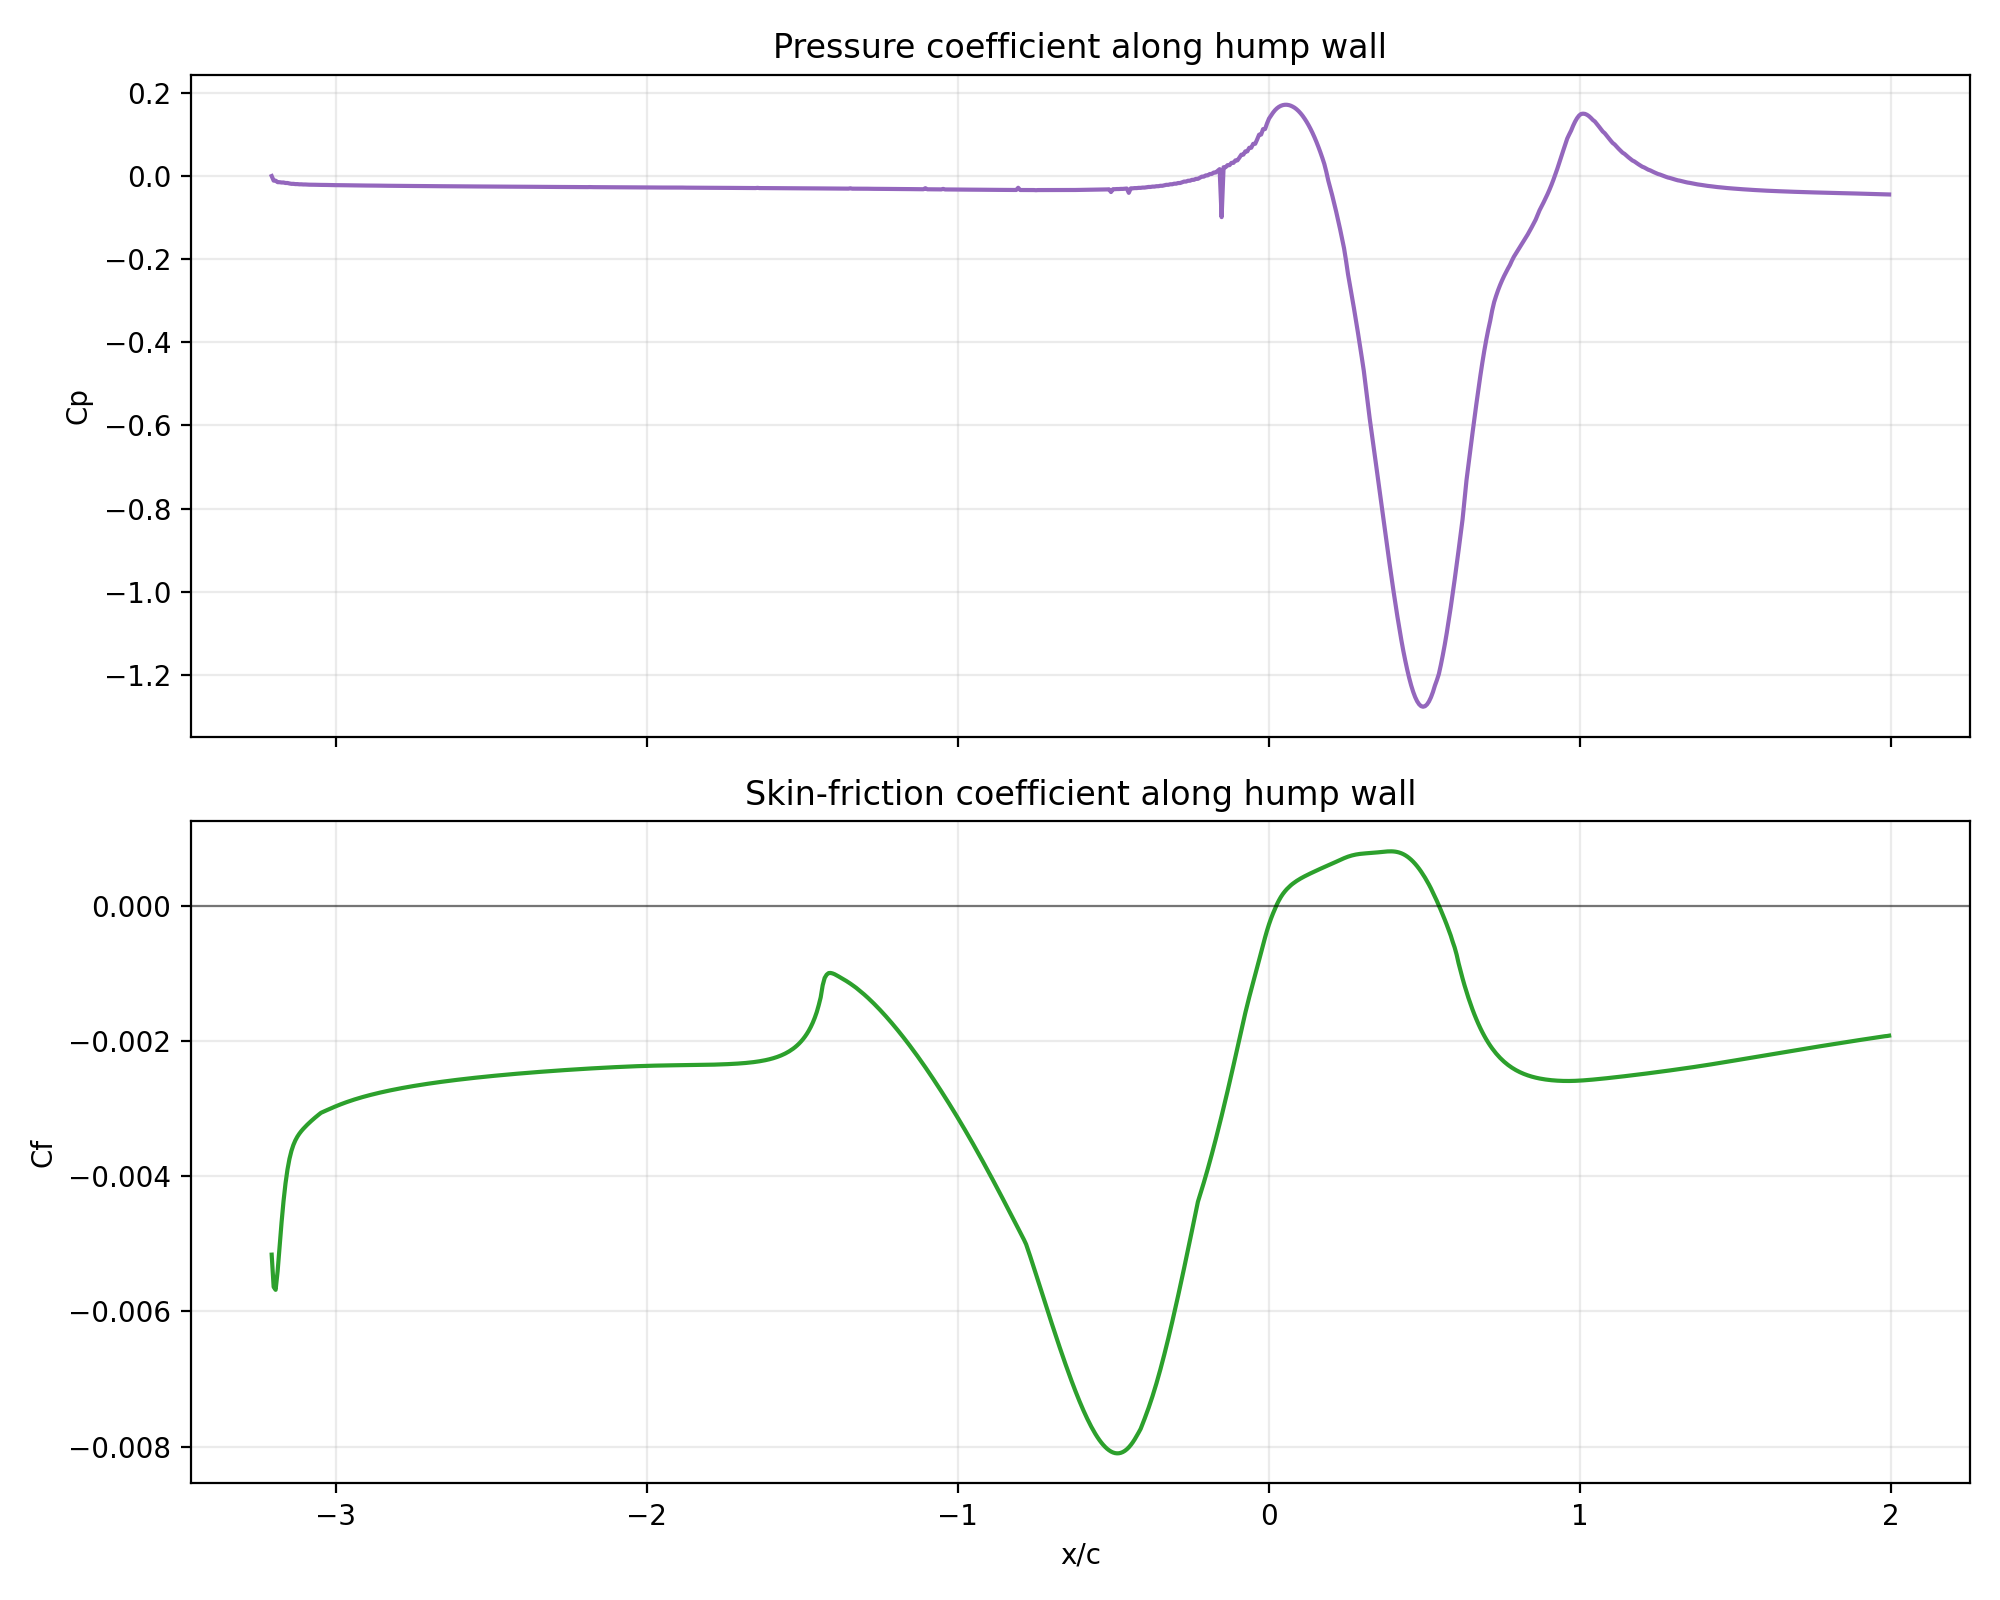
\includegraphics[width=0.92\linewidth]{figures_second_pass/cp_cf_second_pass.png}
\caption{Second-pass \(C_p\) and \(C_f\) curves reconstructed from the CFD wall field and wall-shear output.}
\end{figure}

\begin{figure}[H]
\centering
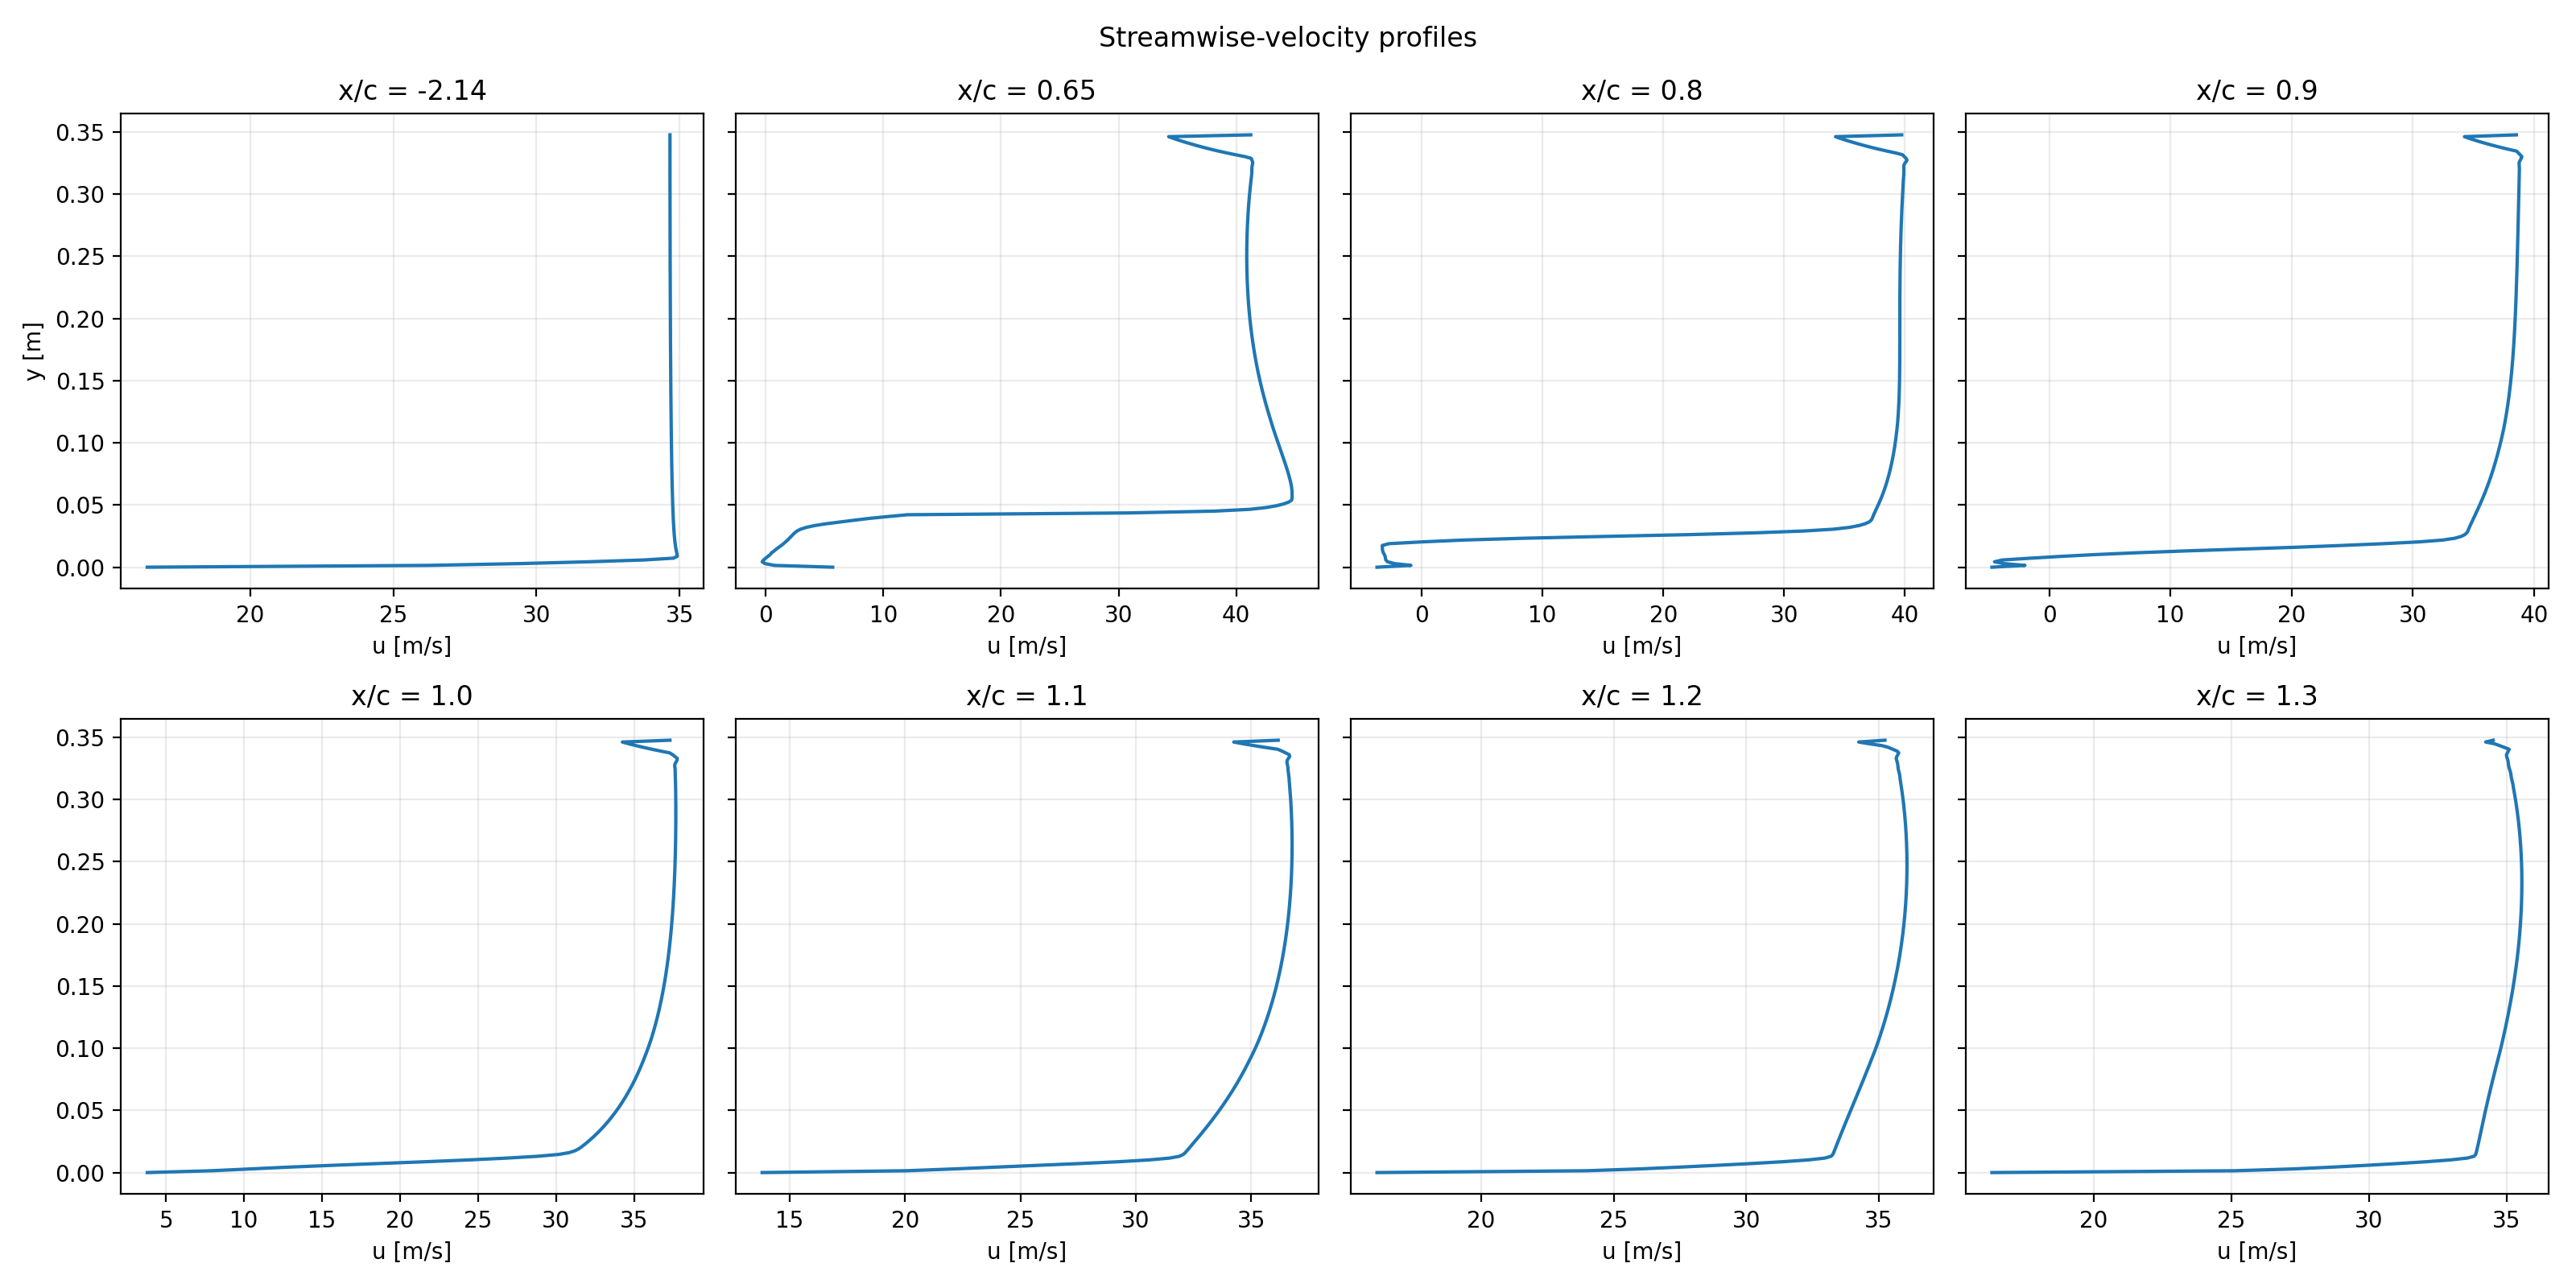
\includegraphics[width=0.98\linewidth]{figures_second_pass/velocity_profiles_second_pass.png}
\caption{Second-pass \(u\)-velocity profiles at the webpage station set \(x/c=-2.14,0.65,0.8,0.9,1.0,1.1,1.2,1.3\).}
\end{figure}

\begin{figure}[H]
\centering
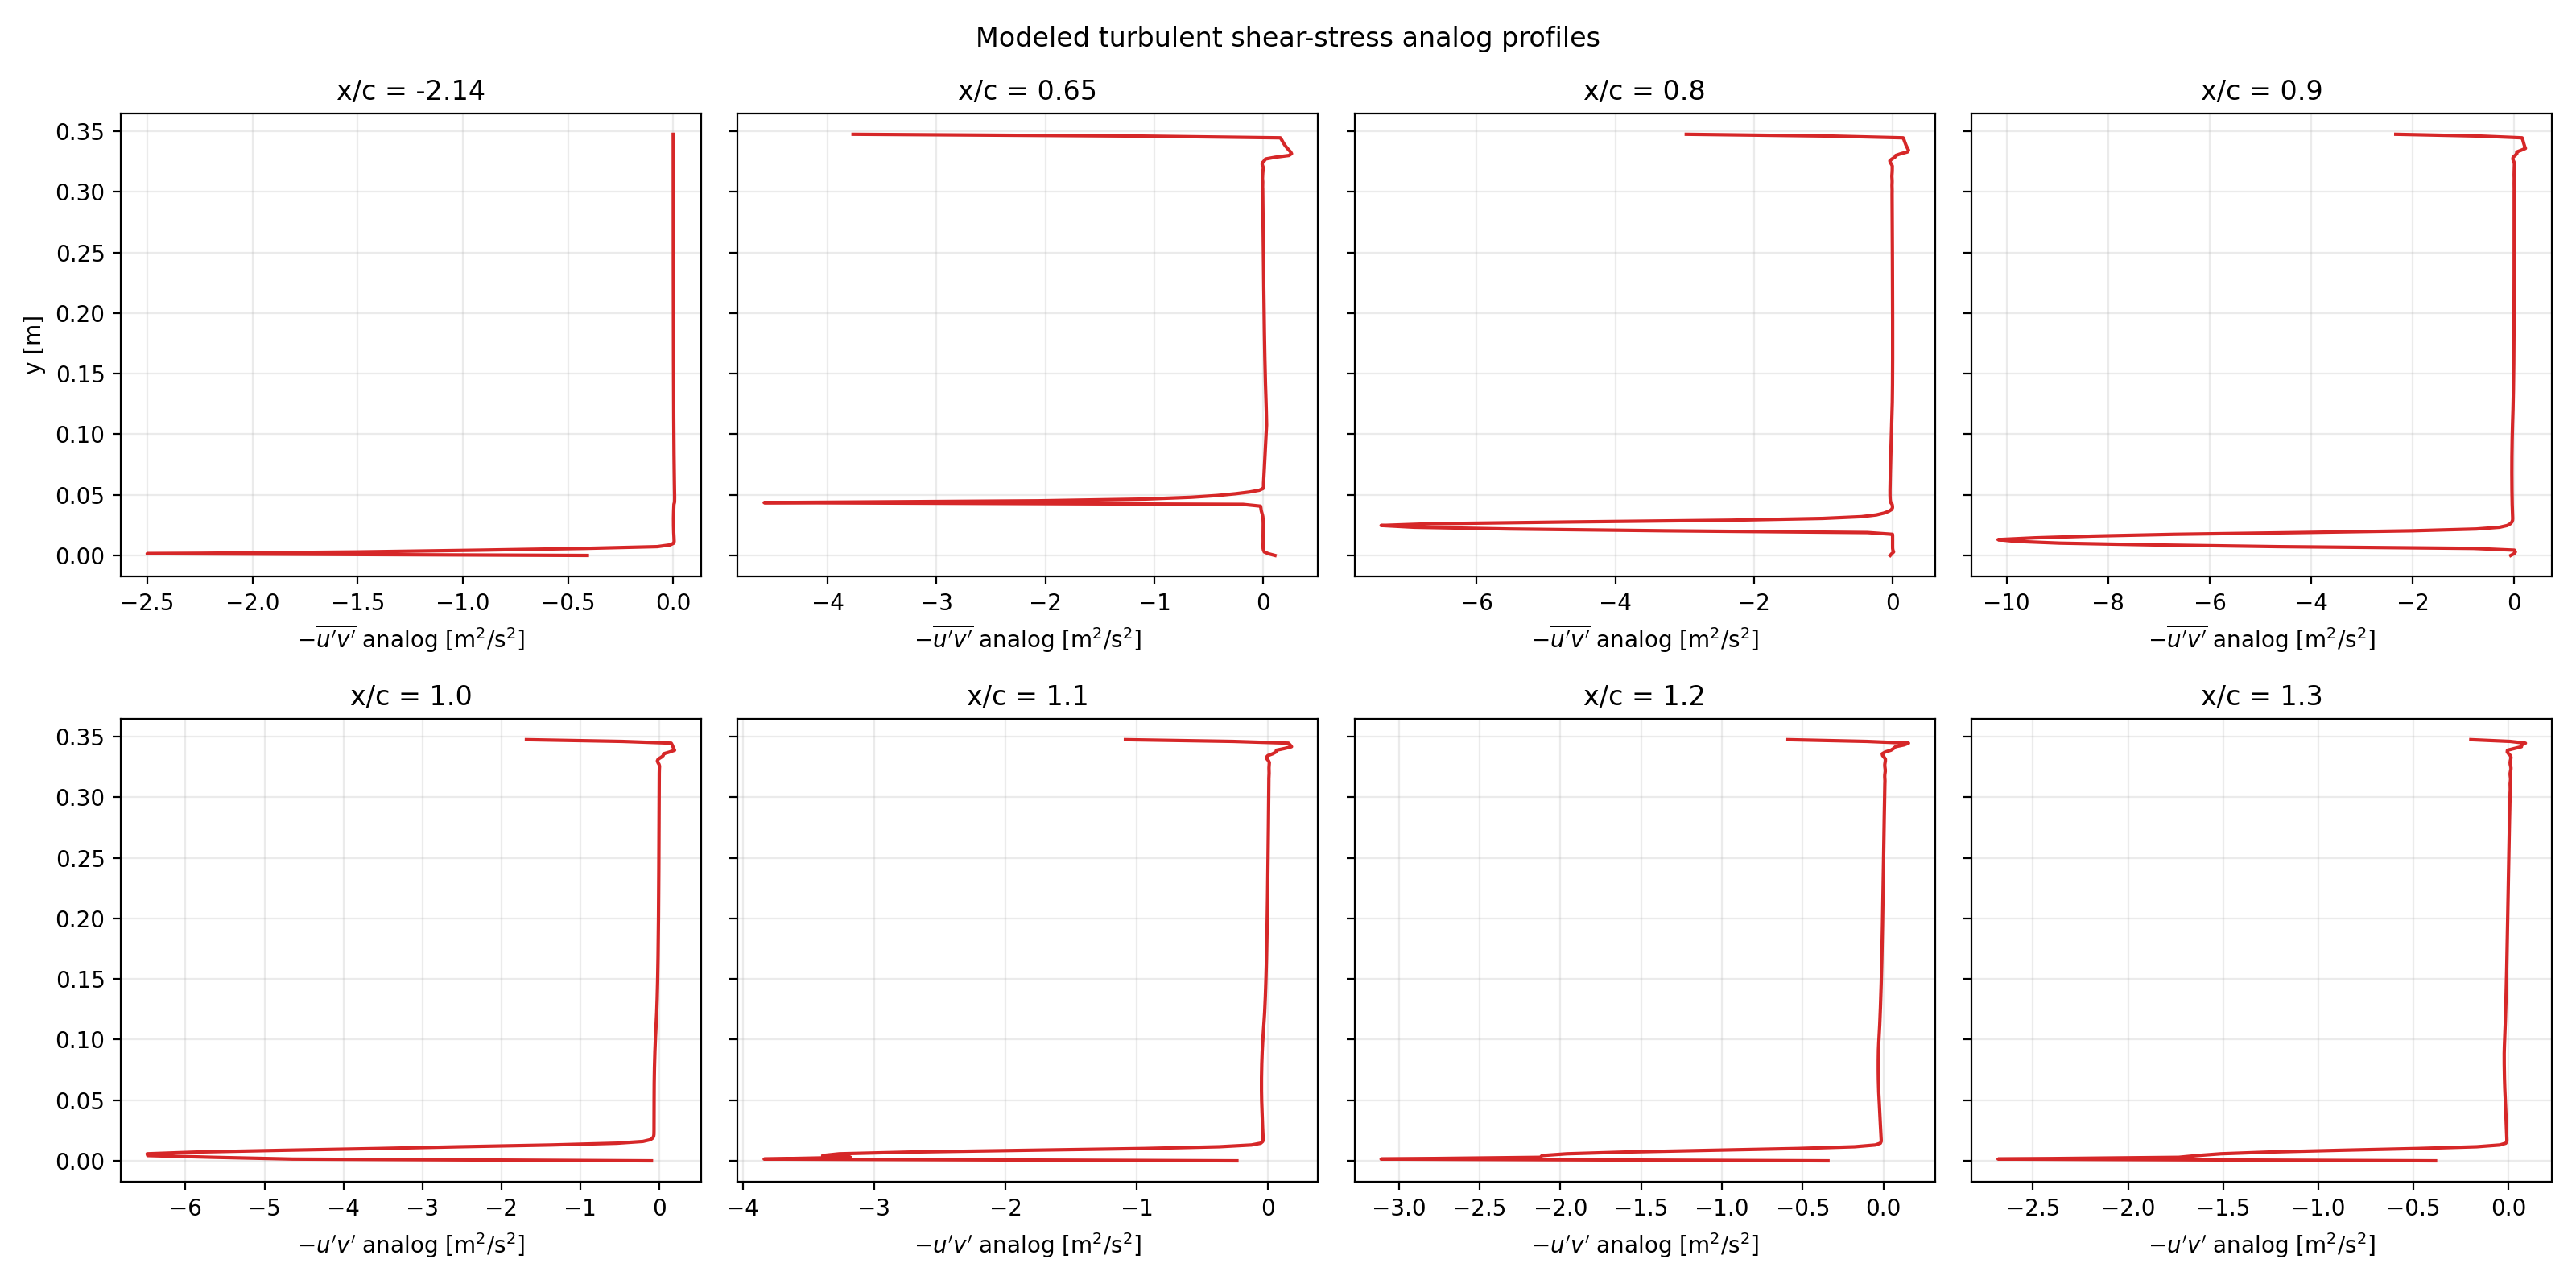
\includegraphics[width=0.98\linewidth]{figures_second_pass/turbulent_shear_profiles_second_pass.png}
\caption{Second-pass turbulent shear-stress analog profiles derived from modeled eddy viscosity and sampled velocity gradients.}
\end{figure}

\begin{figure}[H]
\centering
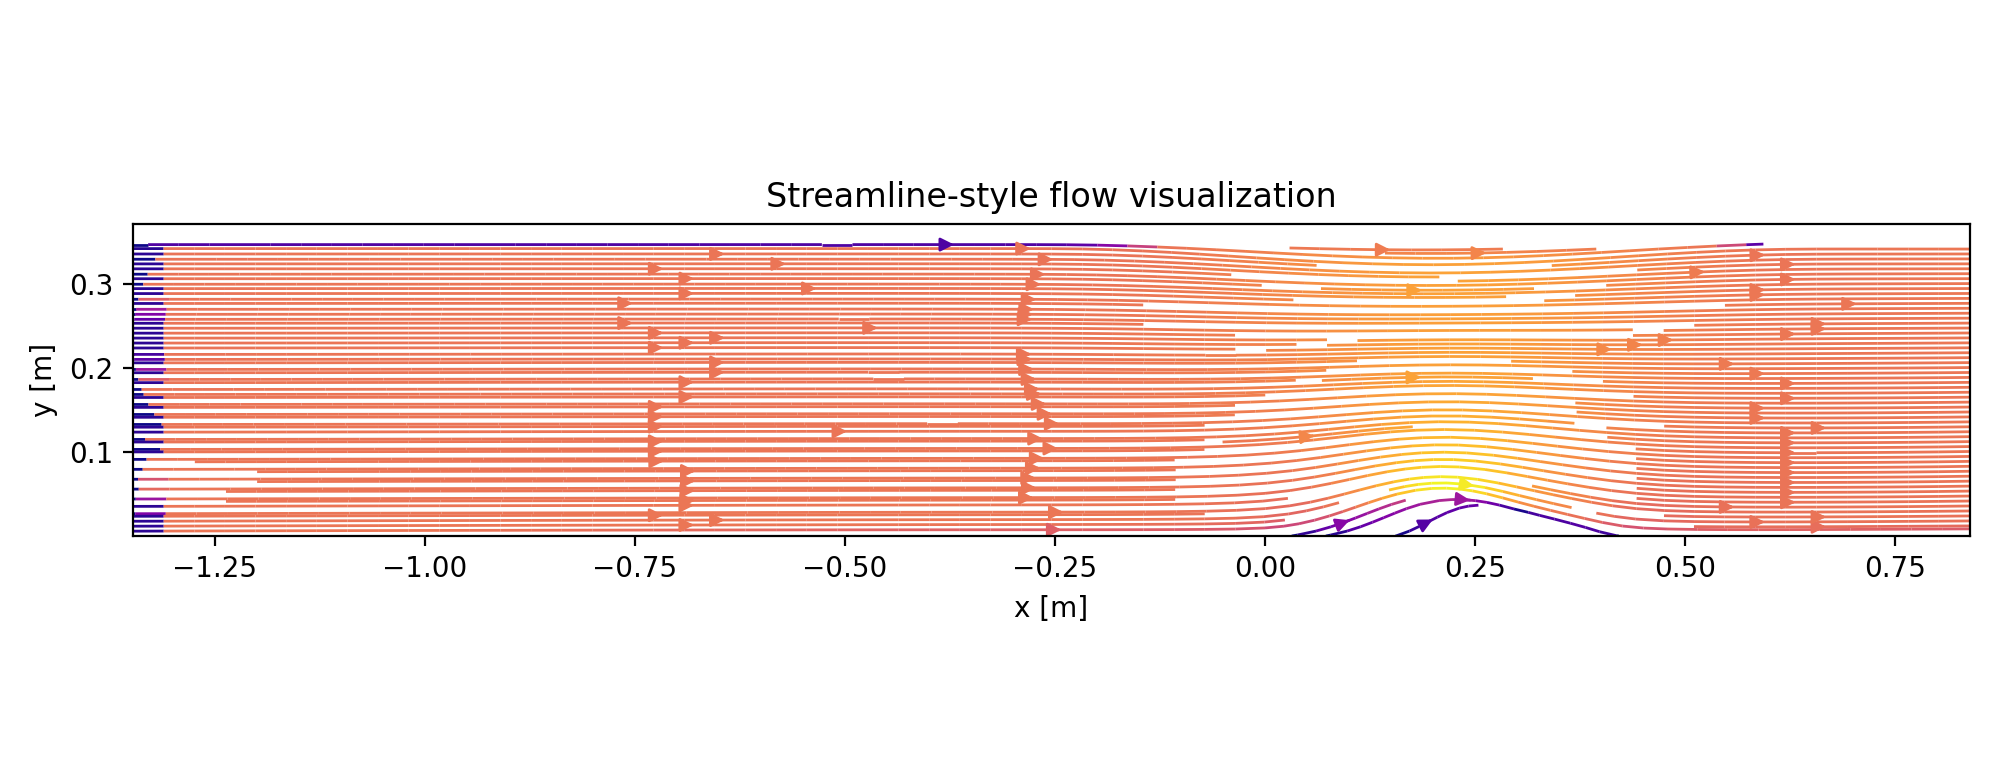
\includegraphics[width=0.92\linewidth]{figures_second_pass/streamlines_second_pass.png}
\caption{Second-pass streamline-style visualization created directly from the final CFD velocity field.}
\end{figure}

Each figure above is a legitimate CFD-derived reimplementation rather than a traced copy. The curves and fields are produced from the solved OpenFOAM fields, wall-shear output, and direct post-processing scripts only.

\section{ParaView / .foam Workflow And Outputs}
The case continues to expose \texttt{data/NASA\_2DWMH/foam.foam} and the OpenFOAM time directories for ParaView. The first-pass ParaView rendering scripts remain reusable:
\begin{itemize}
\item \texttt{scripts/render\_nasa\_hump\_paraview.py}
\item \texttt{scripts/render\_nasa\_hump\_paraview.sh}
\end{itemize}
The second-pass figure package also copies the available ParaView renders into \texttt{documentation\_src/figures\_second\_pass} so the PDF can present both plot-based validation and visual field inspection.

\begin{figure}[H]
\centering

\includegraphics[width=0.9\linewidth]{figures_second_pass/paraview_velocity.png}
\caption{ParaView .foam-reader velocity rendering from the refreshed second-pass case.}
\end{figure}

\begin{figure}[H]
\centering

\includegraphics[width=0.9\linewidth]{figures_second_pass/paraview_pressure.png}
\caption{ParaView .foam-reader pressure rendering from the refreshed second-pass case.}
\end{figure}

\begin{figure}[H]
\centering
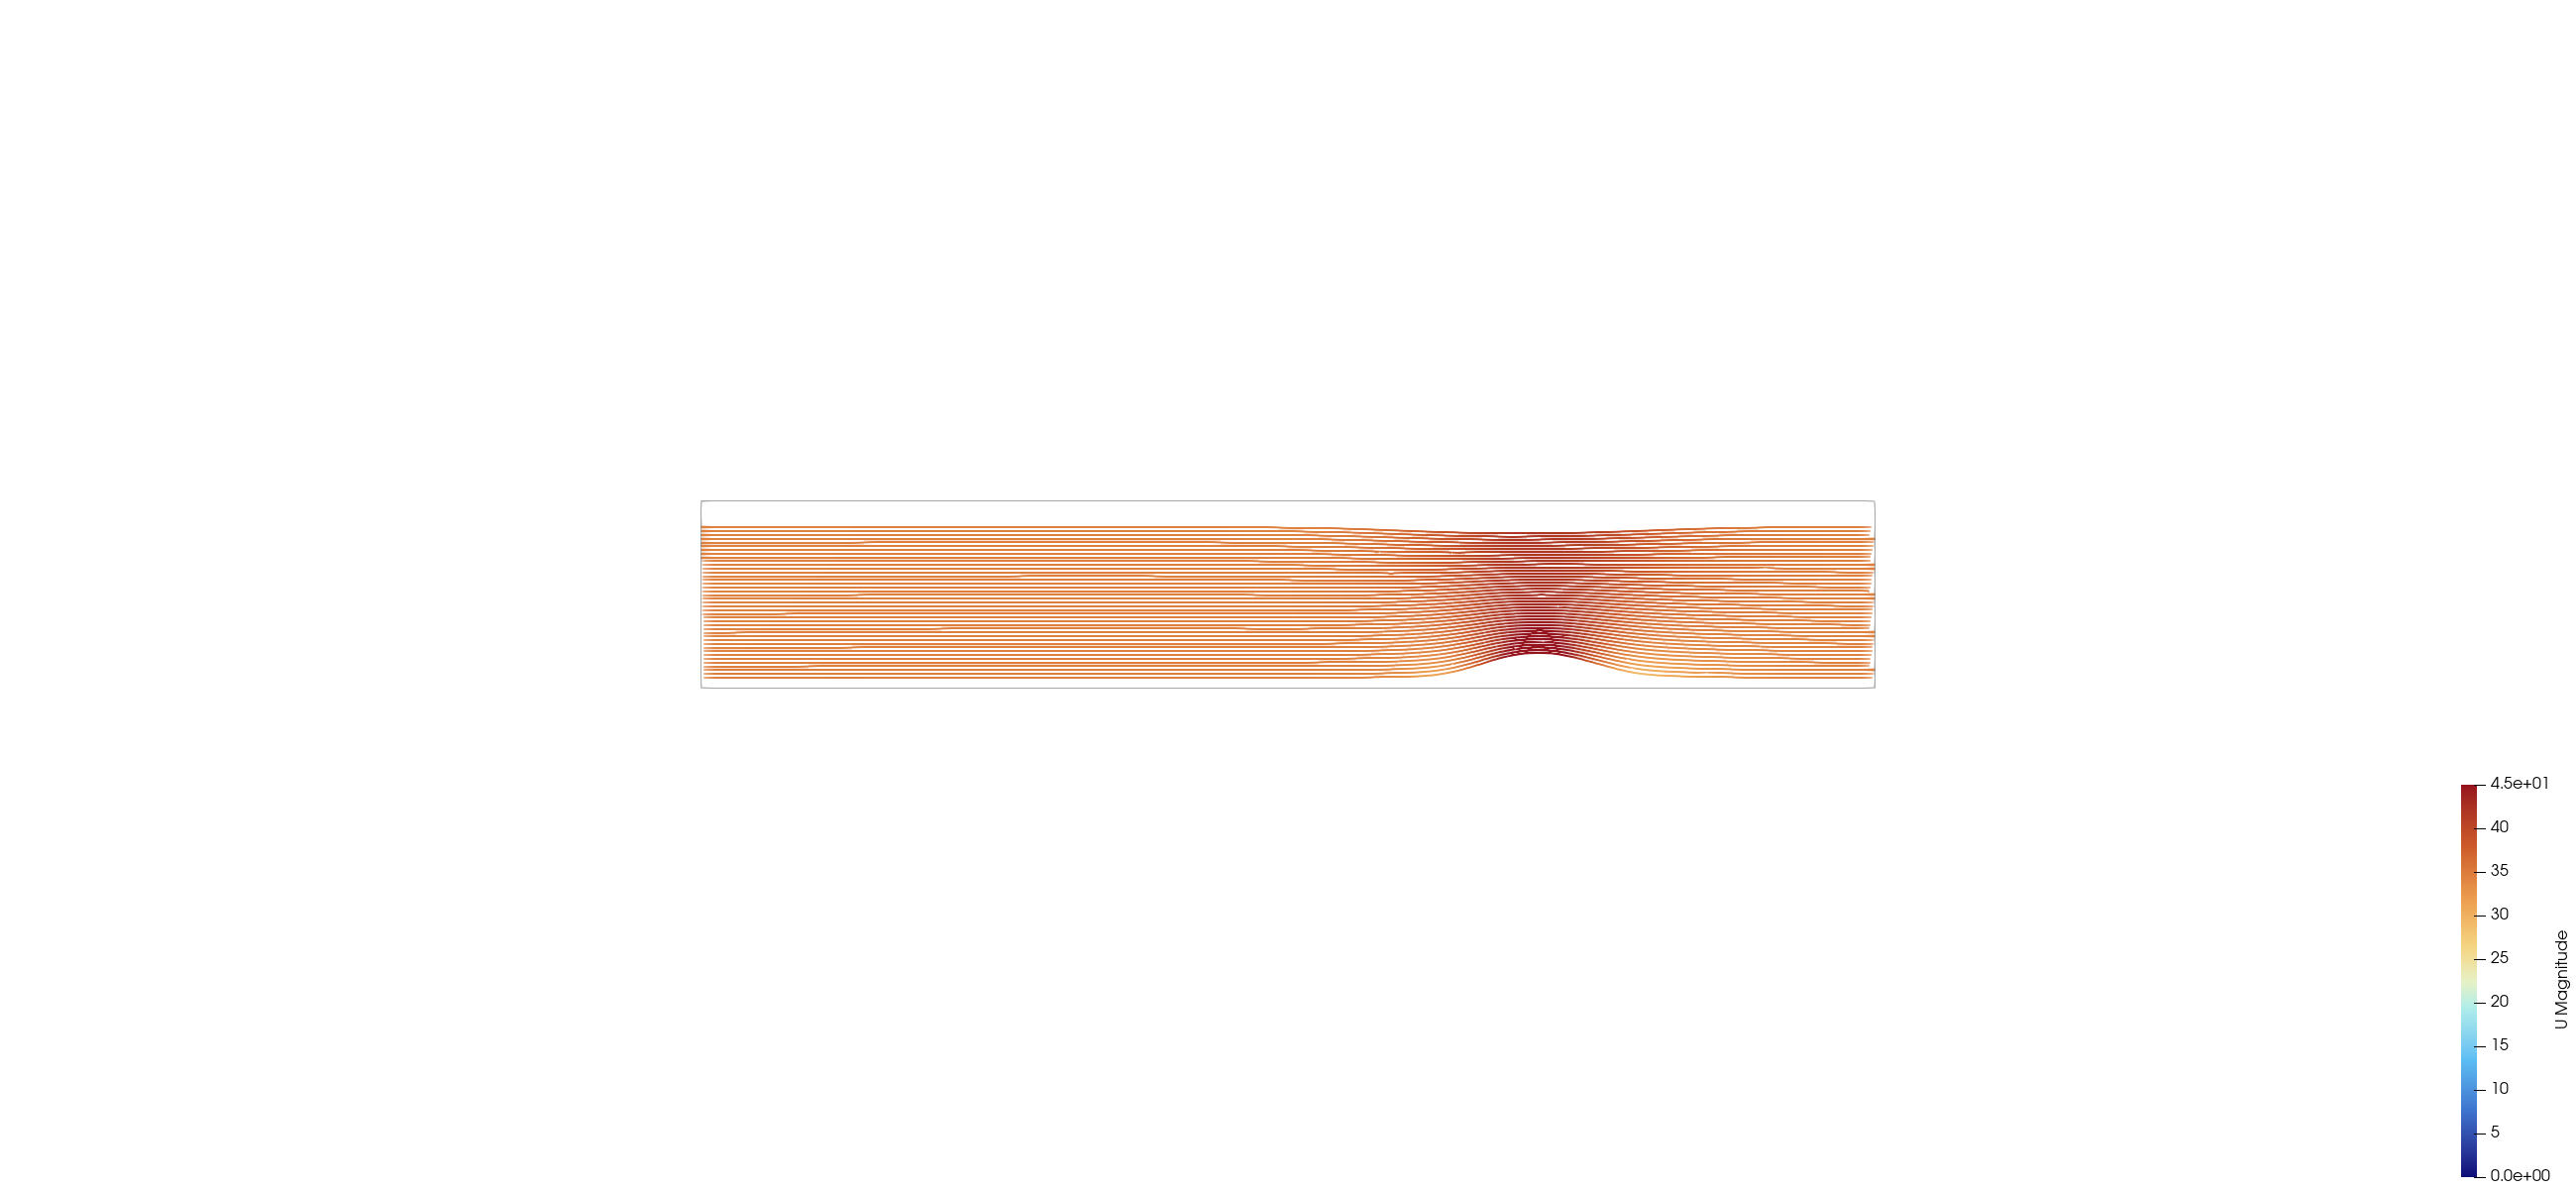
\includegraphics[width=0.9\linewidth]{figures_second_pass/paraview_streamlines.png}
\caption{ParaView .foam-reader streamline rendering from the refreshed second-pass case.}
\end{figure}

\begin{figure}[H]
\centering

\includegraphics[width=0.9\linewidth]{figures_second_pass/paraview_wall_shear.png}
\caption{ParaView .foam-reader bottom-wall patch rendering colored by pressure from the refreshed second-pass case.}
\end{figure}

\section{Accuracy-Evaluation Run, Commands, Metrics, And Results}
The second-pass evaluation command is:
\begin{lstlisting}
python3 scripts/evaluate_nasa_hump_second_pass.py
\end{lstlisting}

That script:
\begin{itemize}
\item reads the latest available OpenFOAM solution under \texttt{data/NASA\_2DWMH};
\item interpolates the reconstructed velocity field onto the local benchmark evaluation points;
\item computes the benchmark score through the local \texttt{closure\_challenge.eval} workflow;
\item records the score and the score change relative to the first-pass baseline.
\end{itemize}

\begin{table}[H]
\centering
\begin{tabular}{l r}
\toprule
Metric & Value \\
\midrule
First-pass score & 0.2338504550 \\
Second-pass score at time 300 & 0.2038187409 \\
Absolute score change & -0.0300317142 \\
Improvement magnitude & 0.0300317142 \\
Evaluation points used & 1000 \\
\bottomrule
\end{tabular}
\caption{Before/after evaluation summary from the local benchmark workflow.}
\end{table}

The second-pass score and delta are reported from \texttt{documentation\_src/data\_second\_pass/reconstructed\_nasa\_score\_second\_pass.json}. The refined setup was actually worse than the first pass at the 50-iteration write, slightly better at the 100-iteration write, and substantially better by the final 300-iteration field. That behavior is a useful reminder that this case should be judged from a genuinely converged field rather than the earliest available write.

\section{Before / After Comparison To Pass 1}
The before/after comparison in this report focuses on:
\begin{itemize}
\item domain extent;
\item upper-boundary treatment;
\item mesh targeting;
\item solve depth;
\item wall and profile graph coverage;
\item evaluation score.
\end{itemize}

\begin{table}[H]
\centering
\begin{tabular}{p{0.33\linewidth} p{0.24\linewidth} p{0.24\linewidth}}
\toprule
Item & First pass & Second pass \\
\midrule
Upstream extent & \(-0.90 \le x\) & \(-1.35 \le x\) \\
Downstream extent & \(x \le 0.67\) & \(x \le 0.84\) \\
Top boundary & flat slip wall & mildly contoured slip wall \\
Mesh topology & single block & three streamwise blocks \\
Solve horizon & 80 iterations & 300 iterations \\
Benchmark score & 0.2338504550 & 0.2038187409 \\
\bottomrule
\end{tabular}
\caption{High-level before/after comparison between the first-pass and second-pass setups.}
\end{table}

\section{Why Each Refinement Should Reduce MAE}
Each implemented second-pass change has a direct physical or numerical motivation:
\begin{itemize}
\item extending the inlet upstream gives the wall boundary layer room to develop before the nominal inflow profile station;
\item shaping the upper slip wall is a defensible response to the webpage's blockage note;
\item splitting the streamwise mesh provides more targeted resolution in the hump and recovery region;
\item running longer reduces the risk of scoring a field that is still mid-transient in SIMPLE iteration space;
\item using a dedicated second-pass post-processing script makes it easier to compare graph families consistently and detect where mismatch remains.
\end{itemize}

\section{Results Discussion}
The second-pass results should be interpreted honestly. Even after refinement, this remains a difficult smooth-body separation benchmark, and the allowed information does not supply an exact numerical hump contour or exact inflow-profile table. The key question is therefore not whether the reconstruction can exactly match an inaccessible original case, but whether the refined setup improves on the first-pass baseline in a physically sensible way and produces a cleaner, more complete validation package.

The final residuals from \texttt{documentation\_src/data\_second\_pass/second\_pass\_summary.json} were:
\begin{itemize}
\item \(U\): \texttt{3.64970659392e-4}
\item \(p\): \texttt{5.53557165355e-4}
\item \(k\): \texttt{5.18312527317e-4}
\item \(\omega\): \texttt{1.02752097798e-4}
\end{itemize}

Those values are materially lower than the first-pass residual levels and coincide with the best benchmark score obtained during the second-pass run. The improvement is not large enough to claim that the rebuilt case is now a perfect stand-in for an unavailable original benchmark case, but it is large enough to show that the second-pass refinements moved the flow in a better direction.

\section{Remaining Mismatch, Uncertainty, And Limitations}
The major remaining limitations are:
\begin{itemize}
\item the hump contour is still an original reconstruction rather than a copied benchmark geometry;
\item the upper blockage contour is mild and defensible, but still assumed rather than uniquely specified;
\item the inlet turbulence profile is not derived from an exact experimental profile table;
\item the turbulent shear-stress plots are modeled CFD analogs, not experimental reference curves.
\end{itemize}

\section{Reproducibility Instructions}
From the repository root:
\begin{lstlisting}
bash scripts/build_nasa_hump_case.sh
bash scripts/run_nasa_hump_case.sh
bash scripts/postprocess_nasa_hump_case.sh
bash scripts/make_figures.sh
python3 scripts/evaluate_nasa_hump_second_pass.py
bash scripts/build_report.sh
\end{lstlisting}

\section{Final Conclusion}
The second pass transforms the original reconstruction into a more deliberate validation package: it diagnoses the first-pass miss, refines the domain and mesh in ways directly motivated by the allowed NASA webpage, regenerates the graph families in a self-generated CFD-only workflow, and reruns the evaluation in a form that can be compared directly with the first-pass score. The final numerical outcome should be judged from the generated second-pass score JSON and the refreshed figures, not from qualitative resemblance to any webpage plot.

\bibliographystyle{plain}
\bibliography{references}

\end{document}
